\documentclass[../main-physics-problems.tex]{subfiles}
\begin{document}

\subsection{Oscillating Motion}

\subsubsection{Changes in an Oscillating Medium}

\subsubsection{Amplitude, Frequency, and Period in Simple Harmonic Motion (SHM)}

\subsubsection{Effects of Changing the Medium and Energy on SHM}

\clearpage

\subsection{Transverse Waves}

\subsubsection{Amplitude, Wavelength, Frequency, and Wave Speed}

\begin{questions}

\begin{EnvUplevel}
    \textbf{Questions \ref{first}--\ref{fifth}.} Count the number of wave cycles. Measurements of wave cycles may be as small as $\frac{1}{4}$ of a cycle.
\end{EnvUplevel}

\question \label{first}
Number of wave cycles: \fillin[7]


\begin{center}
\begin{tikzpicture}[x=3mm,y=1cm]
\draw[black!20,ultra thin,xstep=pi/2,ystep=0.5] (0,-1) grid (16*pi,1);
\draw[domain=pi:pi + 7*2*pi,samples=200] plot (\x,{sin(\x r)});
\ifprintanswers
    \color{red}
    \draw[domain=pi:pi + 2*pi,smooth,ultra thick] plot (\x,{sin(\x r)});
    \fill (3*pi,0) circle (2pt) node [above right] {1};
    \fill (5*pi,0) circle (2pt) node[above right] {2};
    \fill (7*pi,0) circle (2pt) node[above right] {3};
    \fill (9*pi,0) circle (2pt) node[above right] {4};
    \fill (11*pi,0) circle (2pt) node[above right] {5};
    \fill (13*pi,0) circle (2pt) node[above right] {6};
    \fill (15*pi,0) circle (2pt) node[above right] {7};
\fi
\end{tikzpicture}
\end{center}

\question
Number of wave cycles: \fillin[5]

\begin{center}
\begin{tikzpicture}[x=3mm,y=1cm]
\draw[black!20,ultra thin,xstep=pi/2,ystep=0.5] (-pi,-1) grid (11*pi,1);
\draw[domain=0:5*2*pi,samples=200] plot (\x,{sin(\x r)});
\ifprintanswers
    \color{red}
    \draw[domain=0:2*pi,smooth,ultra thick] plot (\x,{sin(\x r)});
    \fill (2*pi,0) circle (2pt) node [above left] {1};
    \fill (4*pi,0) circle (2pt) node [above left] {2};
    \fill (6*pi,0) circle (2pt) node [above left] {3};
    \fill (8*pi,0) circle (2pt) node [above left] {4};
    \fill (10*pi,0) circle (2pt) node [above left] {5};
\fi
\end{tikzpicture}
\end{center}


\question
Number of wave cycles: \fillin[8.75]


\begin{center}
\begin{tikzpicture}[x=2.5mm,y=1cm]
\draw[black!20,ultra thin,xstep=pi/2,ystep=0.5] (-pi/2,-1) grid (19*pi,1);
\draw[domain=0.5*pi:0.5*pi + 8.75*2*pi,samples=200] plot (\x,{sin(\x r)});
\ifprintanswers
    \color{red}
    \draw[domain=0.5*pi:0.5*pi + 2*pi,smooth,ultra thick] plot (\x,{sin(\x r)});
    \fill (2.5*pi,1) circle (2pt) node [above=2pt] {1};
    \fill (4.5*pi,1) circle (2pt) node [above=2pt] {2};
    \fill (6.5*pi,1) circle (2pt) node [above=2pt] {3};
    \fill (8.5*pi,1) circle (2pt) node [above=2pt] {4};
    \fill (10.5*pi,1) circle (2pt) node [above=2pt] {5};
    \fill (12.5*pi,1) circle (2pt) node [above=2pt] {6};
    \fill (14.5*pi,1) circle (2pt) node [above=2pt] {7};
    \fill (16.5*pi,1) circle (2pt) node [above=2pt] {8};
    \draw[domain=0.5*pi + 8*2*pi:0.5*pi + 8.75*2*pi,smooth,ultra thick] plot (\x,{sin(\x r)});
    \fill (0.5*pi+8.75*2*pi,0) circle (2pt) node [above=2pt] {8.75};
\fi
\end{tikzpicture}
\end{center}


\question
Count the total number of wave cycles. Then measure the amplitude and wavelength in grid units.

Number of wave cycles: \fillin[3][1cm] \hfill Amplitude: \fillin[2 units] \hfill Wavelength: \fillin[8 units]

\begin{center}
\begin{tikzpicture}[x=6mm,y=1cm]
\draw[black!20,ultra thin,xstep=0.25*pi,ystep=0.5] (0.25*pi,-1) grid ++(4*2*pi,2);    
\draw[domain=1.5*pi:1.5*pi + 3*2*pi,samples=200] plot (\x,{sin(\x r)});
\ifprintanswers
    \color{red}
    \draw[domain=1.5*pi:1.5*pi + 2*pi,smooth,ultra thick] plot (\x,{sin(\x r)});
\fi
\end{tikzpicture}
\end{center}



\question \label{fifth}
Count the total number of wave cycles. Then measure the amplitude and wavelength in grid units.

Number of wave cycles: \fillin[3.75][1cm] \hfill Amplitude: \fillin[10 units] \hfill Wavelength: \fillin[?]

\begin{center}
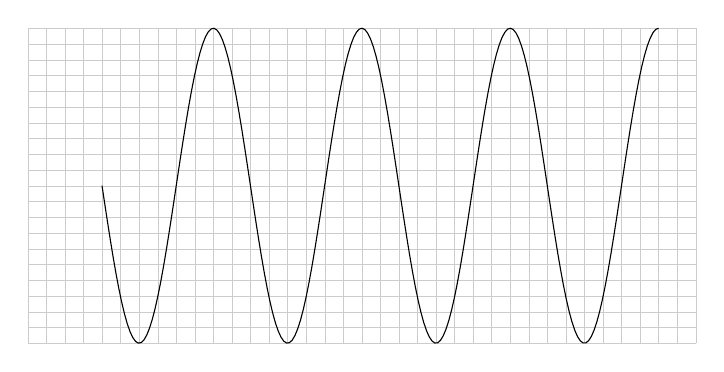
\begin{tikzpicture}[x=3mm,y=2cm]
\draw[black!20,ultra thin,xstep=0.25*pi,ystep=0.1] (0,-1) grid (4.5*2*pi,1);    
\draw[black!20,ultra thin] (0,-1) -- ++(4.5*2*pi,0);    
\draw[domain=pi:pi + 3.75*2*pi,samples=200] plot (\x,{sin(\x r)});
\end{tikzpicture}
\end{center}





\question
Go to \texttt{PhET Simulation: Wave on a String} (\href{https://phet.colorado.edu/sims/html/wave-on-a-string/latest/wave-on-a-string_all.html}{click here}). Set a wave to oscillate with no end, with damping set to none, and with the display of the rulers and timer, as summarized below. Leave all other settings at their default values.

\begin{center}
\begin{minipage}{0.15\textwidth}
\begin{itemize}
    \item[$\bigcirc$] Manual 
    \item[$\bigodot$] \textbf{Oscillate}
    \item[$\bigcirc$] Pulse
\end{itemize}
\end{minipage}%
\hspace{1ex}
\begin{minipage}{0.3\textwidth}
\centering
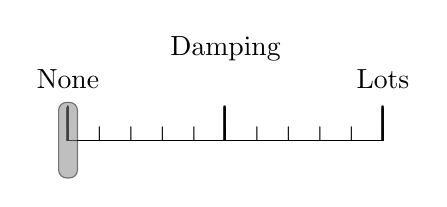
\begin{tikzpicture}[x=4mm,y=4mm]
    \begin{scope}
        \draw (0,0) -- (10,0);
        \clip (-0.5,0) -- (10.5,0) -- (10.5,1.2) -- (0,1.2) -- cycle;
        \foreach \i in {0,1,...,10}{
            \draw (\i,0) node {$|$};
        }
        \foreach \i in {0,5,10}{
            \draw (\i,0) node {\Huge $|$};
        }
    \end{scope}
    \node[above=1.5em] at (0,0) {None};
    \node[above=2.5em] at (5,0) {Damping};
    \node[above=1.5em] at (10,0) {Lots};
    \draw[rounded corners=1mm,fill=black!50,opacity=0.5] (-0.3,-1.2) rectangle (0.3,1.2);
\end{tikzpicture}
\end{minipage}%
\hspace{1ex}
\begin{minipage}{0.15\textwidth}
\centering
\begin{itemize}
    \item[$\bigcirc$] Fixed End 
    \item[$\bigcirc$] Loose End
    \item[$\bigodot$] \textbf{No End}
\end{itemize}
\end{minipage}%
\hspace{1ex}
\begin{minipage}{0.2\textwidth}
\begin{itemize}
    \item[\checkbox{1}] Rulers
    \item[\checkbox{1}] Timer
    \item[$\square$] Reference Line
\end{itemize}
\end{minipage}
\end{center}

\bigskip

For each of the parts below use the play (\faPlay), pause (\faPause), and step (\faStepForward) buttons and the \texttt{Slow Motion} setting as needed to facilitate your measurements.

\begin{parts}

\part
\textit{Measuring amplitude.} The dashed line is the vertical center of the wave and represents the equilibrium position. The amplitude is measured as the vertical distance between the dashed line and the crest, as shown below.

\begin{center}
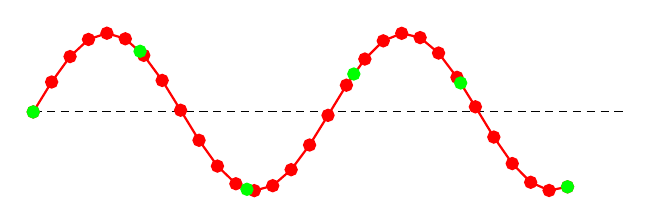
\begin{tikzpicture}
    \draw[densely dashed,x=6mm] (0,0) -- (2*2*pi,0);
    \draw[x=6mm,y=1cm,domain=0:1.8*2*pi,samples=30,thick,red,mark=*] plot (\x,{sin(\x r)});
    \draw[x=6mm,y=1cm,domain=0:1.8*2*pi,samples=6,thick,green,mark=*,only marks] plot (\x,{sin(\x r)});
    \begin{scope}[scale=0.5,shift={(1.9,0)}]
        \tkzRegle[Rotation=90,Longueur=4,AfficheValeurs=false,CouleurFond=white,Opacite=0.5,Fond=true]
    \end{scope}
\end{tikzpicture}
\end{center}

Use the vertical ruler to measure the amplitude: \fillin[0.75]\ cm

\part
\textit{Measuring wavelength.} The wavelength of a wave may be measured as the horizontal distance between two adjacent crests. 

\begin{center}
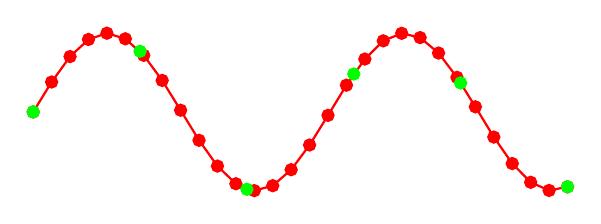
\begin{tikzpicture}
    \draw[x=6mm,y=1cm,domain=0:1.8*2*pi,samples=30,thick,red,mark=*] plot (\x,{sin(\x r)});
    \draw[x=6mm,y=1cm,domain=0:1.8*2*pi,samples=6,thick,green,mark=*,only marks] plot (\x,{sin(\x r)});
    \begin{scope}[scale=0.5,shift={(2,3.8)}]
        \tkzRegle[Longueur=7.5,AfficheValeurs=false,CouleurFond=white,Opacite=1,Fond=true]
    \end{scope}
\end{tikzpicture}
\end{center}

Use the ruler to measure the wavelength: \fillin[4.2]\ cm

\part 
\textit{Measuring frequency and period.} Pause (\faPause) the wave, and step (\faStepForward) it forward so that a crest is exactly aligned at the window frame, as shown below. The window represents a reference point in space, so each time a new crest passes through the window, a wave cycle has been completed.

\begin{center}
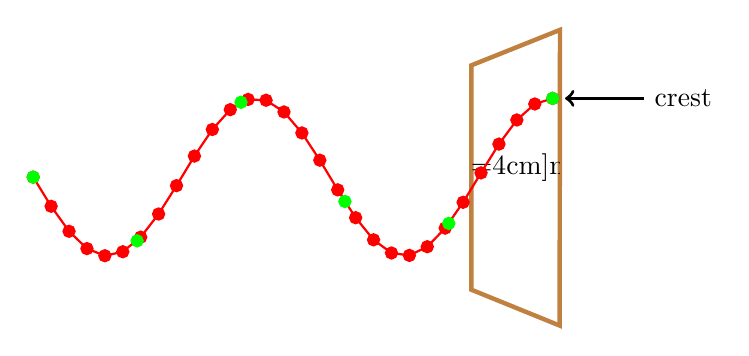
\begin{tikzpicture}
    \begin{scope}[shift={(7.45,-1.43)},x=5mm,y=5mm]]
    \draw[ultra thick,brown] (0,0) -- (0,5.7) -- (2.25,6.6) -- (2.24,-0.91) -- cycle;
    \clip (0,0) -- (0,5.7) -- (2.25,6.6) -- (2.24,-0.91) -- cycle;
    \node at (2,3.1) {\twemoji[height=4cm]{national park}};
    \end{scope}
    \draw[x=6mm,y=1cm,domain=pi:2.25*2*pi,samples=30,thick,red,mark=*] plot (\x,{sin(\x r)});
    \draw[x=6mm,y=1cm,domain=pi:2.25*2*pi,samples=6,thick,green,mark=*,only marks] plot (\x,{sin(\x r)});
    \draw[<-,very thick] (2.75*pi,1) -- ++(1,0) node[right] {crest};
\end{tikzpicture}
\end{center}


Press both the reset and the play buttons on the timer (note that it won't run until the simulation is played). Now play (\faPlay) the simulation and record the time it takes 10 subsequent crests to pass through the window (that's 10 wave cycles). Switching to \texttt{Slow Motion} and using step (\faStepForward) may be useful. Record the time below.

\begin{center}
    Time for 10 wave cycles: \fillin[6.67]\ seconds
\end{center}

Frequency may be defined as wave cycles per second, so divide the number of waves (10) by the total time. Show your work and record the frequency below.

\ifprintanswers
\begin{equation*}
    f = \frac{\textcolor{red}{10}\ \text{wave cycles}}{\textcolor{red}{6.67}\ \mathrm{s}} = \boxed{\textcolor{red}{1.50}\ \mathrm{Hz}}
\end{equation*}
\else
\begin{equation*}
    f = \frac{\textcolor{white}{10}\ \text{wave cycles}}{\textcolor{white}{6.67}\ \mathrm{s}} = \boxed{\textcolor{white}{1.50}\ \mathrm{Hz}}
\end{equation*}
\fi

Similarly, the period ($T$) of the wave is the time it takes to complete one cycle. Using the same data, calculate the wave's period by dividing the total time for 10 wave cycles by the number of cycles (10):


\ifprintanswers
\begin{equation*}
    T = \frac{\textcolor{red}{6.67}\ \mathrm{s}}{\textcolor{red}{10}\ \text{wave cycles}} = \boxed{\textcolor{red}{0.667}\ \mathrm{s}}
\end{equation*}
\else
\begin{equation*}
    T = \frac{\textcolor{white}{6.67}\ \mathrm{s}}{\textcolor{white}{10}\ \text{wave cycles}} = \boxed{\textcolor{white}{0.667}\ \mathrm{s}}
\end{equation*}
\fi

\part
\textit{Measuring wave speed.} Pause (\faPause) and step (\faStepForward) the wave so that a crest aligns with the \SI{0}{cm} mark, as shown below.

\begin{center}
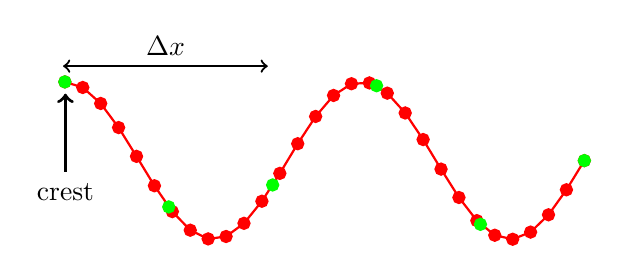
\begin{tikzpicture}
    \draw[x=6mm,y=1cm,domain=pi/2:2*2*pi,samples=30,thick,red,mark=*] plot (\x,{sin(\x r)});
    \draw[x=6mm,y=1cm,domain=pi/2:2*2*pi,samples=6,thick,green,mark=*,only marks] plot (\x,{sin(\x r)});
    \draw[very thick,<-] (0.95,0.85) -- ++(0,-1) node[below] {crest};
    \draw[thick,<->] (0.92,1.2) -- ++(2.6,0) node[above,pos=0.5] {$\Delta x$};
    \begin{scope}[scale=0.87,shift={(1.05,3.5)}]
        \tkzRegle[Longueur=8,AfficheValeurs=true,CouleurFond=white,Opacite=1,Fond=true]
    \end{scope}
\end{tikzpicture}
\end{center}

Reset and play the timer. Then use the \texttt{Slow Motion}, play, and step buttons to record the time it takes the crest to travel exactly \SI{3.0}{cm}. Record this time interval below:

\ifprintanswers
\begin{equation*}
    \Delta t = \textcolor{red}{0.48}\ \mathrm{s}
\end{equation*}
\else
\begin{equation*}
    \Delta t = \textcolor{white}{0.48}\ \mathrm{s}
\end{equation*}
\fi

Speed $(v)$ is distance over time, so fill in the equation below and calculate the wave speed:

\ifprintanswers
\bgroup
\large 
\begin{equation*}
    v = \frac{\Delta x}{\Delta t} = \frac{\textcolor{red}{3.0}\ \mathrm{cm}}{\textcolor{red}{0.48}\ \mathrm{s}} = \boxed{\textcolor{red}{6.25}\ \mathrm{cm/s}}
\end{equation*}
\egroup
\else
\bgroup
\large 
\begin{equation*}
    v = \frac{\Delta x}{\Delta t} = \frac{\textcolor{white}{3.0}\ \mathrm{cm}}{\textcolor{white}{0.48}\ \mathrm{s}} = \boxed{\textcolor{white}{6.25}\ \mathrm{cm/s}}
\end{equation*}
\egroup
\fi
\end{parts}

\question
Amplitude is most closely related which of the following wave properties?

\begin{randomizechoices}
    \correctchoice energy
    \choice wavelength
    \choice frequency
    \choice wave speed
\end{randomizechoices}

\question \label{XGViXs}
The period of a wave is measured to be 4.85 seconds. What is the wave's frequency?


\begin{solution}
\SI{0.206}{Hz}
\end{solution}




\question \label{EeHAB4} 
If the frequency of a wave is 8.53 hertz, what is its period of oscillation?


\begin{solution}
\SI{0.117}{s}
\end{solution}

\question \label{ldTSm3} 
A bead on a string oscillates between a crest and trough of a transverse wave. The bead completes 20 cycles in 16 seconds. Calculate the wave's average period of oscillation. 


\begin{solution}
\SI{0.8}{s}
\end{solution}

\question \label{3rLSIq}
What is the frequency of the wave described in Exercise \ref{ldTSm3}?


\begin{solution}
\SI{1.25}{Hz}
\end{solution}

\question \label{gz0LQL} 
Every second, a transverse wave completes exactly five and four-sevenths of a wave cycle. Calculate the period of oscillation.


\begin{solution}
\SI{0.179}{s}
\end{solution}

\question \label{MITNpN} 
Electromagnetic (EM) waves are transverse (but not mechanical) waves that oscillate at high frequencies. One type of EM waves is the radio wave, like those use detected by your car. Calculate the frequency of a radio wave whose period of oscillation is a tiny \SI[group-separator={\,}]{0.0001814}{s}.


\begin{solution}
    \SI{5513}{Hz}
\end{solution}

\question
What two physical quantities are needed to calculate the velocity of a wave?


\question \label{SKv3ek}
The following wave has a frequency of \SI{2.70}{Hz} and propagates to the right. What is the velocity of the wave?


\begin{center}
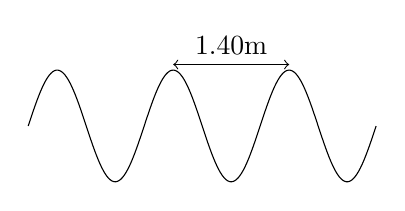
\begin{tikzpicture}
\begin{axis}[width=6cm,height=3cm,
    xmin=0,xmax=3*2,
    ymin=-1,ymax=1,
    clip=false,
    ticks=none,
    axis line style={draw=none}]
    \draw plot[domain=0:3*2*pi, samples=200] (\x/pi,{sin(\x r)});
    \draw[<->] (2.5,1.1) -- ++(axis direction cs: 2,0) node[above,pos=0.5] {\SI{1.40}{m}};
\end{axis}
\end{tikzpicture}
\end{center}


\question \label{HcdmDZ}
The wave below has a period of 11 seconds as it propagates rightwards. Calculate its wave velocity.

\begin{center}
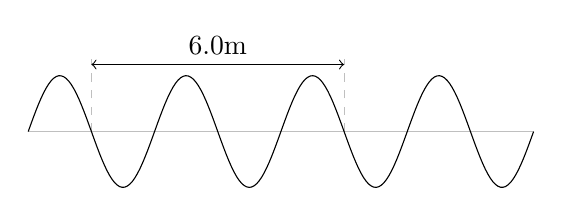
\begin{tikzpicture}
\begin{axis}[width=8cm,height=3cm,
    xmin=0,xmax=4*2,
    ymin=-1,ymax=1,
    clip=false,
    ticks=none,
    axis line style={draw=none}]
    \draw[lightgray] (0,0) -- (4*2,0);
    \draw[lightgray,dashed] (1,0) -- ++(axis direction cs: 0,1.3) (5,0) -- ++(axis direction cs: 0,1.3);
    \draw plot[domain=0:4*2*pi, samples=200] (\x/pi,{sin(\x r)});
    \draw[<->] (1,1.2) -- ++(axis direction cs: 4,0) node[above,pos=0.5] {\SI{6.0}{m}};
\end{axis}
\end{tikzpicture}
\end{center}


\question \label{exdA2j}
Calculate the velocity of a wave whose wavelength and period of oscillation are \SI{10.5}{m} and \SI{0.25}{s}, respectively. 


\question \label{HoRqxe}
What is the velocity of a wave whose frequency and wavelength are \SI{25}{Hz} and \SI{7.0}{m}, respectively?


\question
Access the \texttt{PhET Simulation} ``Waves Intro'' (\href{https://phet.colorado.edu/sims/html/waves-intro/latest/waves-intro_en.html}{click here}). Click the \texttt{Light} panel. 

\begin{enumerate}
\setlength\itemsep{0.1ex}
    \item Press the \texttt{green} button on the laser to emit green light waves.
    \item Click and drag the ruler tool from the upper-right-hand corner to measure the horizontal distance from the center of one bright spot to the next. \textbf{Tip}: by default, the ruler is set the measure the wavelength of green light.
    \item Convert the given measurement from nanometers (nm) to meters (m), given that $\SI{1}{nm} = 10^{-9}\,\text{m}$.
    \item If the wave travels at a speed of 300 million meters per second (\SI{3e8}{m/s}), what is the frequency of the light wave? Express the answer both in scientific notation and in decimal notation.
\end{enumerate}




\end{questions}


\subsubsection{Effects of Changing the Medium on Transverse Waves}
\begin{questions}

\question
Go to \texttt{PhET Simulation: Wave on a String} (\href{https://phet.colorado.edu/sims/html/wave-on-a-string/latest/wave-on-a-string_all.html}{click here}). Set a wave to oscillate with no end, with damping set to none, and with the display of the rulers and timer, as summarized below. Leave all other settings at their default values.

\begin{center}
\begin{minipage}{0.15\textwidth}
\begin{itemize}
    \item[$\bigcirc$] Manual 
    \item[$\bigodot$] \textbf{Oscillate}
    \item[$\bigcirc$] Pulse
\end{itemize}
\end{minipage}%
\hspace{1ex}
\begin{minipage}{0.3\textwidth}
\centering
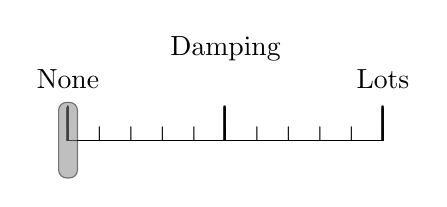
\begin{tikzpicture}[x=4mm,y=4mm]
    \begin{scope}
        \draw (0,0) -- (10,0);
        \clip (-0.5,0) -- (10.5,0) -- (10.5,1.2) -- (0,1.2) -- cycle;
        \foreach \i in {0,1,...,10}{
            \draw (\i,0) node {$|$};
        }
        \foreach \i in {0,5,10}{
            \draw (\i,0) node {\Huge $|$};
        }
    \end{scope}
    \node[above=1.5em] at (0,0) {None};
    \node[above=2.5em] at (5,0) {Damping};
    \node[above=1.5em] at (10,0) {Lots};
    \draw[rounded corners=1mm,fill=black!50,opacity=0.5] (-0.3,-1.2) rectangle (0.3,1.2);
\end{tikzpicture}
\end{minipage}%
\hspace{1ex}
\begin{minipage}{0.15\textwidth}
\centering
\begin{itemize}
    \item[$\bigcirc$] Fixed End 
    \item[$\bigcirc$] Loose End
    \item[$\bigodot$] \textbf{No End}
\end{itemize}
\end{minipage}%
\hspace{1ex}
\begin{minipage}{0.2\textwidth}
\begin{itemize}
    \item[\checkbox{1}] Rulers
    \item[\checkbox{1}] Timer
    \item[$\square$] Reference Line
\end{itemize}
\end{minipage}
\end{center}

In a previous problem, we found that the default wave speed is \SI{6.25}{cm/s}.

\begin{parts}
\part Increase the amplitude to \SI{1.25}{cm}. Then, as previously done, record the time it takes for a crest to be horizontally displaced by \SI{3}{cm}, and use the average velocity equation to find wave speed:

\ifprintanswers
\begin{equation*}
    v = \frac{\Delta x}{\Delta t} = \frac{\textcolor{red}{3.0}\ \mathrm{cm}}{\textcolor{red}{0.48}\ \mathrm{s}} = \boxed{\textcolor{red}{6.25}\ \mathrm{cm/s}}
\end{equation*}
\else
\begin{equation*}
    v = \frac{\Delta x}{\Delta t} = \frac{\textcolor{white}{3.0}\ \mathrm{cm}}{\textcolor{white}{0.48}\ \mathrm{s}} = \boxed{\textcolor{white}{6.25}\ \mathrm{cm/s}}
\end{equation*}
\fi

How does increasing amplitude affect the transverse wave speed?

\ifprintanswers
\else
\fillwithlines{1.5cm}
\fi

\begin{solution}
    Increasing the amplitude does not affect wave speed. It only affects the energy transported by the wave.
\end{solution}

\part
Reset the amplitude back to the default, \SI{0.75}{cm}. Then change the tension in the string to low:

\begin{center}
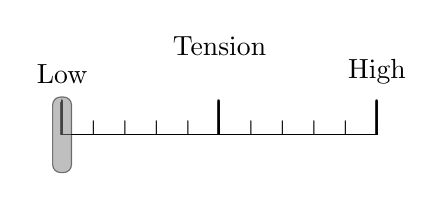
\begin{tikzpicture}[x=4mm,y=4mm]
    \begin{scope}
        \draw (0,0) -- (10,0);
        \clip (-0.5,0) -- (10.5,0) -- (10.5,1.2) -- (0,1.2) -- cycle;
        \foreach \i in {0,1,...,10}{
            \draw (\i,0) node {$|$};
        }
        \foreach \i in {0,5,10}{
            \draw (\i,0) node {\Huge $|$};
        }
    \end{scope}
    \node[above=1.5em] at (0,0) {Low};
    \node[above=2.5em] at (5,0) {Tension};
    \node[above=1.5em] at (10,0) {High};
    \draw[rounded corners=1mm,fill=black!50,opacity=0.5] (-0.3,-1.2) rectangle (0.3,1.2);
\end{tikzpicture}
\end{center}


Once again, record the time it takes for a crest to be horizontally displaced by \SI{3}{cm}, and find the wave speed:

\ifprintanswers
\begin{equation*}
    v = \frac{\Delta x}{\Delta t} = \frac{\textcolor{red}{3.0}\ \mathrm{cm}}{\textcolor{red}{2.38}\ \mathrm{s}} = \boxed{\textcolor{red}{1.26}\ \mathrm{cm/s}}
\end{equation*}
\else
\begin{equation*}
    v = \frac{\Delta x}{\Delta t} = \frac{\textcolor{white}{3.0}\ \mathrm{cm}}{\textcolor{white}{2.38}\ \mathrm{s}} = \boxed{\textcolor{white}{1.26}\ \mathrm{cm/s}}
\end{equation*}
\fi

How does decreasing the tension in the string affect the wave speed? Conversely, how might increasing tension affect wave speed?

\ifprintanswers
\else
\fillwithlines{1.5cm}
\fi

\begin{solution}
    Decreasing string tension also decreases the wave speed, and increasing tension increases wave speed.
\end{solution}

\part 
The linear mass density of the string is $\mu = \SI{1.0}{g/cm}$. Calculate the tension in the string when it's set to low. Express the answer in newtons (N).

\begin{solutionorbox}[4cm]
In base SI units, the linear mass density is

\begin{equation*}
    \mu = \SI[per-mode=fraction]{1.0}{\gram\per\centi\meter} \times 
    \frac{\SI{1}{kg}}{\SI{1000}{g}} \times \frac{\SI{100}{cm}}{\SI{1}{m}} = \SI{0.1}{kg/m}
\end{equation*}

The wave speed on a string is related to tension and linear mass density as

\begin{equation*}
    v_\mathrm{string} = \sqrt{\frac{F_\mathrm{T}}{\mu}}
\end{equation*}

Solving for tension leads to

\begin{equation*}
    F_\mathrm{T} = \mu v_\mathrm{string}^2 = (\SI{0.1}{kg/m}) \left(\SI{1.26e-2}{m/s}\right)^2 =  \boxed{\SI{1.6e-5}{N}}
\end{equation*}
\end{solutionorbox}

\part 
Using the same linear mass density from the previous part, find the tension, in newtons, when tension is set to high. 



\begin{solutionorbox}[4cm]
From previous measurements, we know that when tension is high, the string speed is $v_\mathrm{string} = \SI{6.25}{cm/s} = \SI{6.25e-2}{m/s}$. Using the result from the previous part, tension is

\begin{equation*}
    F_\mathrm{T} = \mu v_\mathrm{string}^2 = (\SI{0.1}{kg/m}) \left(\SI{6.25e-2}{m/s}\right)^2 =  \boxed{\SI{3.9e-4}{N}}
\end{equation*}
\end{solutionorbox}

\end{parts}

\end{questions}
\clearpage


\subsubsection{Mathematical Relationship between Frequency, Wave Velocity, and Wavelength}

\begin{questions}
\question
The sinusoidal wave function is

\begin{equation*}
    y(x,t) = A \sin\left(\frac{2\pi x}{\lambda} - 2\pi f t\right)
\end{equation*}


Graphing this as a function of position ($x$) and time ($t$) can be very illuminating. 

\begin{parts}

\part Go to \href{https://www.desmos.com/calculator}{desmos.com/calculator} and define the following variables and their limits:

\begin{align*}
    A &= 2 \qquad 0.1 \leq A \leq 8 \\[1ex]
    \lambda &= 5 \qquad 0.1 \leq \lambda \leq 10 \\[1ex]
    f &= 1 \qquad 0.1 \leq f \leq 3\\[1ex]
    t &= 0 \qquad 0 \leq t \leq 10\\[1ex]
    y(x) &= A \sin\left(\frac{2\pi x}{\lambda} - 2\pi f t\right)
\end{align*}

where $A$, $\lambda$, and $f$ are wave quantities. \textbf{Note:} You need to copy-and-paste the $\lambda$ symbol into Desmos by searching for ``lowercase lambda'' on Google. 

\medskip

Make a graph of what you see in Desmos below.

\begin{center}
\begin{tikzpicture}
\begin{axis}[height=6cm,width=10cm,
    axis lines=center,
    ymin=-4,ymax=4,
    xmin=-10,xmax=10,
    ytick={-6,-4,...,6},
    xtick={-10,-6,...,10},
    minor y tick num=1,
    minor x tick num=1,
    grid=both,
]
    \ifprintanswers
    \addplot[domain=-10:10,samples=125,very thick, red] {2*sin(2*pi/5*deg(x))};
    \fi
\end{axis}
\end{tikzpicture}
\end{center}

\part 
Press the play (\faPlay) button in the cell containing the variable $A$ to animate this variable to different values between 0.1 and 10. How does varying $A$ affect the wave? What wave property does $A$ represent?

\ifprintanswers
\else
\fillwithlines{2.0cm}
\fi

\part
Reset $A$ back to 2. Then press the play (\faPlay) button in the $\lambda$ cell to animate $\lambda$. How does varying $\lambda$ affect the wave? What wave property does $\lambda$ represent?

\ifprintanswers
\else
\fillwithlines{2.0cm}
\fi


\part
Reset $\lambda$ to 5. Now press the play (\faPlay) to animate $f$. What happens?

\ifprintanswers
\else
\fillwithlines{2.0cm}
\fi

\part
Reset $f$ back to 1. Go to the $t=0$ cell, click open the animation properties ($\rightleftarrows$), and set the animation mode to play indefinitely ($\rightarrow$). Then press play (\faPlay) to animate $t$. Using the words ``wave,'' ``propagate,'' and ``wave speed,'' describe what you see in the space below.

\ifprintanswers
\else
\fillwithlines{2.0cm}
\fi

\begin{solution}
    \textit{Answers may vary.}

    The wave propagates to the right with a constant wave speed.
\end{solution}

\part
While $t$ is playing indefinitely, manually set the slider on $f$ to different values between 0.1 and 3. Now what do you notice? What wave quantity does $f$ represent?

\ifprintanswers
\else
\fillwithlines{2.0cm}
\fi

\begin{solution}
    \textit{Answers may vary.}

    It's the frequency. When $f$ increases while $\lambda$ is held constant, the wave speed increases.
\end{solution}

\end{parts}

\end{questions}



\clearpage

\subsubsection{Constructive and Destructive Interference}

\begin{questions}
\question
Go to \href{https://www.desmos.com/calculator}{desmos.com/calculator}. In the first cell, define the variable $t = 0$ with limits from $-5$ to $5$:

\begin{equation*}
    t = 0 \qquad -5 \leq t \leq 5
\end{equation*}

Then define the following functions in cells 2 and 3:

\begin{align*}
    f_1 &= 4 e^{-\left(x-t\right)^2} \\[1ex]
    f_2 &= 4 e^{-\left(x+t\right)^2}
\end{align*}

In cell 1, where $t$ is defined, press the play (\faPlay) button to begin looping $t$ forwards and backwards. Observe the motion of the pulses. Now follow the parts below.

\begin{parts}
\part
Pause the animation at $t = -3$, $-1.5$, $-0.75$, and $0$. Then sketch the waves $f_1$  and $f_2$ below.

\begin{center}
\begin{tikzpicture}
\begin{axis}[height=4.0cm,width=8cm,
    axis lines=center,
    ymin=0,ymax=8,
    xmin=-6,xmax=6,
    ytick={0,2,...,8},
    xtick={-6,-4,...,6},
    grid=both,
]
    \ifprintanswers
    \addplot[domain=-6:6,samples=120,thick, blue] {4*exp(-(x+3)^2)};
    \addplot[domain=-6:6,samples=120,thick, green!50!black] {4*exp(-(x-3)^2)};
    \fi
    \node[below left,fill=white] at (axis description cs: 1,1) {$\boxed{t = -3}$};
\end{axis}
\end{tikzpicture}
\hspace{1cm}
\begin{tikzpicture}
\begin{axis}[height=4.0cm,width=8cm,
    axis lines=center,
    ymin=0,ymax=8,
    xmin=-6,xmax=6,
    ytick={0,2,...,8},
    xtick={-6,-4,...,6},
    grid=both,
]
    \ifprintanswers
    \addplot[domain=-6:6,samples=120,thick, blue] {4*exp(-(x+1.5)^2)};
    \addplot[domain=-6:6,samples=120,thick, green!50!black] {4*exp(-(x-1.5)^2)};
    \fi
    \node[below left,fill=white] at (axis description cs: 1,1) {$\boxed{t = -1.5}$};
\end{axis}
\end{tikzpicture}

\vspace{1mm}

\begin{tikzpicture}
\begin{axis}[height=4.0cm,width=8cm,
    axis lines=center,
    ymin=0,ymax=8,
    xmin=-6,xmax=6,
    ytick={0,2,...,8},
    xtick={-6,-4,...,6},
    grid=both,
]
    \ifprintanswers
    \addplot[domain=-6:6,samples=120,thick, blue] {4*exp(-(x+0.75)^2)};
    \addplot[domain=-6:6,samples=120,thick, green!50!black] {4*exp(-(x-0.75)^2)};
    \fi
    \node[below left,fill=white] at (axis description cs: 1,1) {$\boxed{t = -0.75}$};
\end{axis}
\end{tikzpicture}
\hspace{1cm}
\begin{tikzpicture}
\begin{axis}[height=4.0cm,width=8cm,
    axis lines=center,
    ymin=0,ymax=8,
    xmin=-6,xmax=6,
    ytick={0,2,...,8},
    xtick={-6,-4,...,6},
    grid=both,
]
    \ifprintanswers
    \addplot[domain=-6:6,samples=120,thick, blue] {4*exp(-(x)^2)};
    \addplot[domain=-6:6,samples=120,thick, green!50!black] {4*exp(-(x)^2)};
    \fi
    \node[below left,fill=white] at (axis description cs: 1,1) {$\boxed{t = 0}$};
\end{axis}
\end{tikzpicture}
\end{center}

\part 
If cell 4, define the function $f_3 = f_1 + f_2$. Play (\faPlay) the $t$ cell to begin the loop, and pause and sketch $f_3$ at the same times below.

\begin{center}
\begin{tikzpicture}
\begin{axis}[height=4.0cm,width=8cm,
    axis lines=center,
    ymin=0,ymax=8,
    xmin=-6,xmax=6,
    ytick={0,2,...,8},
    xtick={-6,-4,...,6},
    grid=both,
]
    \ifprintanswers
    \addplot[domain=-6:6,samples=120,thick, red] {4*exp(-(x-3)^2) + 4*exp(-(x+3)^2)};
    \fi
    \node[below left,fill=white] at (axis description cs: 1,1) {$\boxed{t = -3}$};
\end{axis}
\end{tikzpicture}
\hspace{1cm}
\begin{tikzpicture}
\begin{axis}[height=4.0cm,width=8cm,
    axis lines=center,
    ymin=0,ymax=8,
    xmin=-6,xmax=6,
    ytick={0,2,...,8},
    xtick={-6,-4,...,6},
    grid=both,
]
    \ifprintanswers
    \addplot[domain=-6:6,samples=120,thick, red] {4*exp(-(x-1.5)^2) + 4*exp(-(x+1.5)^2)};
    \fi
    \node[below left,fill=white] at (axis description cs: 1,1) {$\boxed{t = -1.5}$};
\end{axis}
\end{tikzpicture}

\vspace{1mm}

\begin{tikzpicture}
\begin{axis}[height=4.0cm,width=8cm,
    axis lines=center,
    ymin=0,ymax=8,
    xmin=-6,xmax=6,
    ytick={0,2,...,8},
    xtick={-6,-4,...,6},
    grid=both,
]
    \ifprintanswers
    \addplot[domain=-6:6,samples=120,thick,red] {4*exp(-(x-0.75)^2) + 4*exp(-(x+0.75)^2)};
    \fi
    \node[below left,fill=white] at (axis description cs: 1,1) {$\boxed{t = -0.75}$};
\end{axis}
\end{tikzpicture}
\hspace{1cm}
\begin{tikzpicture}
\begin{axis}[height=4.0cm,width=8cm,
    axis lines=center,
    ymin=0,ymax=8,
    xmin=-6,xmax=6,
    ytick={0,2,...,8},
    xtick={-6,-4,...,6},
    grid=both,
]
    \ifprintanswers
    \addplot[domain=-6:6,samples=120,thick, red] {4*exp(-(x)^2) + 4*exp(-(x)^2)};
    \fi
    \node[below left,fill=white] at (axis description cs: 1,1) {$\boxed{t = 0}$};
\end{axis}
\end{tikzpicture}
\end{center}

\part
What behavior do you see when the waves meet at the same location?

% \ifprintanswers
% \else
\fillwithlines{1.5cm}
% \fi
\end{parts}

\question 
Hide the graph $f_3$ by pressing the button in cell 4. Then change the second function to negative, as

\begin{equation*}
    f_2 = -4e^{-(x+t)^2}
\end{equation*}

Then in cell 1, press play (\faPlay) to set $t$ looping forward and backward.

\begin{parts}

\part
Again, pause the animation at $t = -3$, $-1.5$, $-0.75$, and $0$. Then sketch the waves $f_1$  and $f_2$ below.

\begin{center}
\begin{tikzpicture}
\begin{axis}[height=5.0cm,width=8cm,
    axis lines=center,
    ymin=-6,ymax=6,
    xmin=-6,xmax=6,
    ytick={-6,-4,...,6},
    xtick={-6,-4,...,6},
    grid=both,
]
    \ifprintanswers
    \addplot[domain=-6:6,samples=120,thick, blue] {4*exp(-(x+3)^2)};
    \addplot[domain=-6:6,samples=120,thick, green!50!black] {-4*exp(-(x-3)^2)};
    \fi
    \node[below left,fill=white] at (axis description cs: 1,1) {$\boxed{t = -3}$};
\end{axis}
\end{tikzpicture}%
\hspace{2em}
\begin{tikzpicture}
\begin{axis}[height=5.0cm,width=8cm,
    axis lines=center,
    ymin=-6,ymax=6,
    xmin=-6,xmax=6,
    ytick={-6,-4,...,6},
    xtick={-6,-4,...,6},
    grid=both,
]
    \ifprintanswers
    \addplot[domain=-6:6,samples=120,thick, blue] {4*exp(-(x+1)^2)};
    \addplot[domain=-6:6,samples=120,thick, green!50!black] {-4*exp(-(x-1)^2)};
    \fi
    \node[below left,fill=white] at (axis description cs: 1,1) {$\boxed{t = -1}$};
\end{axis}
\end{tikzpicture}

\medskip

\begin{tikzpicture}
\begin{axis}[height=5.0cm,width=8cm,
    axis lines=center,
    ymin=-6,ymax=6,
    xmin=-6,xmax=6,
    ytick={-6,-4,...,6},
    xtick={-6,-4,...,6},
    grid=both,
]
    \ifprintanswers
    \addplot[domain=-6:6,samples=120,thick, blue] {4*exp(-(x+0.3)^2)};
    \addplot[domain=-6:6,samples=120,thick, green!50!black] {-4*exp(-(x-0.3)^2)};
    \fi
    \node[below left,fill=white] at (axis description cs: 1,1) {$\boxed{t = -0.3}$};
\end{axis}
\end{tikzpicture}%
\hspace{2em}
\begin{tikzpicture}
\begin{axis}[height=5.0cm,width=8cm,
    axis lines=center,
    ymin=-6,ymax=6,
    xmin=-6,xmax=6,
    ytick={-6,-4,...,6},
    xtick={-6,-4,...,6},
    grid=both,
]
    \ifprintanswers
    \addplot[domain=-6:6,samples=120,thick, blue] {4*exp(-(x)^2)};
    \addplot[domain=-6:6,samples=120,thick, green!50!black] {-4*exp(-(x)^2)};
    \fi
    \node[below left,fill=white] at (axis description cs: 1,1) {$\boxed{t =0}$};
\end{axis}
\end{tikzpicture}
\end{center}

\part 
Show $f_3$ by pressing the button in cell 4. Then graph $f_3 = f_1 + f_2$ for the same values of $t$ as the previous part. 

\begin{center}
\begin{tikzpicture}
\begin{axis}[height=5.0cm,width=8cm,
    axis lines=center,
    ymin=-6,ymax=6,
    xmin=-6,xmax=6,
    ytick={-6,-4,...,6},
    xtick={-6,-4,...,6},
    grid=both,
]
    \ifprintanswers
    \addplot[domain=-6:6,samples=120,thick, red] {-4*exp(-(x-3)^2) + 4*exp(-(x+3)^2)};
    \fi
    \node[below left,fill=white] at (axis description cs: 1,1) {$\boxed{t = -3}$};
\end{axis}
\end{tikzpicture}
\hspace{1cm}
\begin{tikzpicture}
\begin{axis}[height=5.0cm,width=8cm,
    axis lines=center,
    ymin=-6,ymax=6,
    xmin=-6,xmax=6,
    ytick={-6,-4,...,6},
    xtick={-6,-4,...,6},
    grid=both,
]
    \ifprintanswers
    \addplot[domain=-6:6,samples=120,thick, red] {-4*exp(-(x-1)^2) + 4*exp(-(x+1)^2)};
    \fi
    \node[below left,fill=white] at (axis description cs: 1,1) {$\boxed{t = -1}$};
\end{axis}
\end{tikzpicture}

\vspace{1mm}

\begin{tikzpicture}
\begin{axis}[height=5.0cm,width=8cm,
    axis lines=center,
    ymin=-6,ymax=6,
    xmin=-6,xmax=6,
    ytick={-6,-4,...,6},
    xtick={-6,-4,...,6},
    grid=both,
]
    \ifprintanswers
    \addplot[domain=-6:6,samples=120,thick, red] {-4*exp(-(x-0.3)^2) + 4*exp(-(x+0.3)^2)};
    \fi
    \node[below left,fill=white] at (axis description cs: 1,1) {$\boxed{t = -0.3}$};
\end{axis}
\end{tikzpicture}
\hspace{1cm}
\begin{tikzpicture}
\begin{axis}[height=5.0cm,width=8cm,
    axis lines=center,
    ymin=-6,ymax=6,
    xmin=-6,xmax=6,
    ytick={-6,-4,...,6},
    xtick={-6,-4,...,6},
    grid=both,
]
    \ifprintanswers
    \addplot[domain=-6:6,samples=120,thick, red] {-4*exp(-(x)^2) + 4*exp(-(x)^2)};
    \fi
    \node[below left,fill=white] at (axis description cs: 1,1) {$\boxed{t =0}$};
\end{axis}
\end{tikzpicture}
\end{center}

\part
What behavior do you see when the waves meet at the same location?
% \ifprintanswers
% \else
\fillwithlines{1.5cm}
% \fi

\end{parts}


\question
Go to \href{https://www.desmos.com/calculator}{desmos.com/calculator}. In the first cell, define the variable $t = 0$ with limits from $-5$ to $5$. Then, define wavelength $\lambda$, frequency $f$, and a coefficient $A$ as follows:

\begin{align*}
    & t = 0 \qquad -5 \leq t \leq 5 \\[1ex]
    & \lambda = 2 \\[1ex]
    & A = 0.2 \\[1ex]
    & f = 1
\end{align*}

The pressure wave of a sound as a function of distance from the source may be modeled by a sinusoidal wave function combined with an exponential decay function; define this equation in the next cell:

\begin{equation*}
    f_1 = e^{-Ax} \sin\left(\frac{2\pi x}{\lambda} - 2\pi f t\right)
\end{equation*}

Noise-cancellation technology in headphones works by recording the sound wave of an external source and producing a secondary sound wave in your ear that destructively interferes with the first wave to effectively cancel out the external noise.

In the next cell, write an equation for a function $f_2$ that destructively interferes with sound wave $f_1$. Then plot $f_1 + f_2$ to show that the the first wave was canceled by the second.

\begin{solution}
\begin{equation*}
    f_2 = -e^{-Ax} \sin\left(\frac{2\pi x}{\lambda} - 2\pi f t\right)
\end{equation*}    
\end{solution}

\end{questions}




% Watch ``Wave Machine Demonstration'' by \texttt{National STEM Centre} on \texttt{YouTube} (\href{https://youtu.be/VE520z_ugcU}{click here}).

% \begin{questions}




% \question \label{OIqgoJ}
% Access the \texttt{PhET Simulation} ``Waves on a String'' (\href{https://phet.colorado.edu/en/simulations/wave-on-a-string}{click here}). Then take the following steps two create two pulses.
    
% \begin{enumerate}
% \setlength\itemsep{0.1ex}
%     \item Press the screen (on the play button) to start the simulation.
%     \item Select the \texttt{Pulse} and \texttt{Loose End} options.
%     \item Increase the \texttt{Amplitude} to \SI{1.25}{cm}.
%     \item Decrease the \texttt{Damping} to \texttt{None}.
%     \item Set the \texttt{Tension} to the medium value.
%     \item Click the green pulse button twice, with a 1-second gap between the two clicks.
%     \item When the two pulses overlap on the same side of the equilibrium line (above or below it), what happens to the string?
%     \item When the two pulses are on opposite sides---for example, if one pulse is above the equilibrium line, and the other is below---what happens to the string?
% \end{enumerate}

% \begin{center}
%     \includegraphics[width=12cm]{physics-2023-24/figures/Unit11_PhET_Wave2.png}
% \end{center}


% \begin{solution}
% When two pulses converge on the same side of the equilibrium line, that portion of the string grows in height as the amplitudes of the two pulses add up. However, when pulses that are on opposite sides converge, the string momentarily flattens as the opposite amplitudes of the pulses cancel each other out.
% \end{solution}



% \begin{multicols*}{2}
% \question
% .

% \begin{tikzpicture}[step=1,x=4mm,y=4mm]
%     \draw[lightgray] (0,0) grid (12,24);
%     \draw[gray] (6,0) -- (6,24);
%     \draw[ultra thick,shift={(0,20)}] (0,0) node[left] {$t = 0$} -- (3,0) -- (3,1) -- (5,1) node[pos=0.5,above] {\large $\rightarrow$} -- (5,0) -- (7,0) -- (7,1) -- (9,1) node[pos=0.5,above] {\large $\leftarrow$} -- (9,0) -- (12,0);
%     \node[left] at (0,4) {$t=4$};
%     \node[left] at (0,8) {$t=3$};
%     \node[left] at (0,12) {$t=2$};
%     \node[left] at (0,16) {$t=1$};
%     \ifprintanswers
%         \draw[red,ultra thick,shift={(0,16)}] (0,0) -- (4,0) -- (4,1) -- (6,1) node[above,pos=0.5] {$\rightarrow$} -- (8,1) node[above,pos=0.5] {$\leftarrow$} -- (8,0) -- (12,0);
%         \draw[red, ultra thick,shift={(0,12)}] (0,0) -- (5,0) -- (5,2) -- (6,2) node[above,pos=0.5] {$\rightarrow$} -- (7,2) node[above,pos=0.5] {$\leftarrow$} -- (7,0) -- (12,0);
%         \draw[red,ultra thick,shift={(0,8)}] (0,0) -- (4,0) -- (4,1) -- (6,1) node[above,pos=0.5] {$\leftarrow$} -- (8,1) node[above,pos=0.5] {$\rightarrow$} -- (8,0) -- (12,0);
%         \draw[red,ultra thick,shift={(0,4)}] (0,0) -- (3,0) -- (3,1) -- (5,1) node[pos=0.5,above] {\large $\leftarrow$} -- (5,0) -- (7,0) -- (7,1) -- (9,1) node[pos=0.5,above] {\large $\rightarrow$} -- (9,0) -- (12,0);
%     \fi
% \end{tikzpicture}

% \question
% .

% \begin{tikzpicture}[step=1,x=4mm,y=4mm]
%     \draw[lightgray] (0,0) grid (12,24);
%     \draw[gray] (6,0) -- (6,24);
%     \draw[ultra thick,shift={(0,20)}] (0,0) node[left] {$t = 0$} -- (3,0) -- (3,1) -- (5,1) node[pos=0.5,above] {\large $\rightarrow$} -- (5,0) -- (6,0) -- (7,0) -- (7,-1) -- (9,-1) node[pos=0.5,below] {\large $\leftarrow$} -- (9,0) -- (12,0);
%     \node[left] at (0,4) {$t=4$};
%     \node[left] at (0,8) {$t=3$};
%     \node[left] at (0,12) {$t=2$};
%     \node[left] at (0,16) {$t=1$};
%     \ifprintanswers
%         \draw[red,ultra thick,shift={(0,16)}] (0,0) -- (4,0) -- (4,1) -- (6,1) node[above,pos=0.5] {$\rightarrow$} -- (6,0) -- (6,-1) -- (8,-1) node[below,pos=0.5] {$\leftarrow$} -- (8,0) -- (12,0);
%         \draw[red, ultra thick,shift={(0,12)}] (0,0) -- (12,0);
%         \draw[red,ultra thick,shift={(0,8)}] (0,0) -- (4,0) -- (4,-1) -- (6,-1) node[below,pos=0.5] {$\leftarrow$} -- (6,0) -- (6,1) -- (8,1) node[above,pos=0.5] {$\rightarrow$} -- (8,0) -- (12,0);
%         \draw[red,ultra thick,shift={(0,4)}] (0,0) -- (3,0) -- (3,-1) -- (5,-1) node[pos=0.5,below] {\large $\leftarrow$} -- (5,0) -- (7,0) -- (7,1) -- (9,1) node[pos=0.5,above] {\large $\rightarrow$} -- (9,0) -- (12,0);
%     \fi
% \end{tikzpicture}

% \vspace*{\fill}

% \columnbreak

% \question
% .

% \begin{tikzpicture}[step=1,x=4mm,y=4mm]
%     \draw[lightgray] (0,0) grid (12,24);
%     \draw[gray] (6,0) -- (6,24);
%     \draw[ultra thick,shift={(0,20)}] (0,0) node[left] {$t = 0$} -- (3,0) -- (3,1) -- (4,1) node[pos=0.5,above] {\large $\rightarrow$} -- (4,-1) -- (5,-1) -- (5,0) -- (6,0) -- (7,0) -- (7,-1) -- (8,-1) -- (8,1) -- (9,1) node[pos=0.5,above] {\large $\leftarrow$} -- (9,0) -- (12,0);
%     \node[left] at (0,4) {$t=4$};
%     \node[left] at (0,8) {$t=3$};
%     \node[left] at (0,12) {$t=2$};
%     \node[left] at (0,16) {$t=1$};
%     \ifprintanswers
%         \draw[red,ultra thick,shift={(0,16)}] (0,0) -- (3,0);
%     \fi
% \end{tikzpicture}

% \question
% .

% \begin{tikzpicture}[step=1,x=4mm,y=4mm]
%     \draw[lightgray] (0,0) grid (12,24);
%     \draw[gray] (6,0) -- (6,24);
%     \draw[ultra thick,shift={(0,20)}] (0,0) node[left] {$t = 0$} -- (3,0) -- (3,1) -- (4,1) node[pos=0.5,above] {\large $\rightarrow$} -- (4,-1) -- (5,-1) -- (5,0) -- (6,0) -- (7,0) -- (7,1) -- (8,1) node[pos=0.5,above] {\large $\leftarrow$} -- (8,-1) -- (9,-1)  -- (9,0) -- (12,0);
%     \node[left] at (0,4) {$t=4$};
%     \node[left] at (0,8) {$t=3$};
%     \node[left] at (0,12) {$t=2$};
%     \node[left] at (0,16) {$t=1$};
%     \ifprintanswers
%         \draw[red,ultra thick,shift={(0,16)}] (0,0) -- (3,0);
%     \fi
% \end{tikzpicture}

% \vspace*{\fill}

% \question
% .

% \begin{tikzpicture}[step=1,x=4mm,y=4mm]
%     \draw[lightgray] (0,0) grid (12,24);
%     \draw[gray] (6,0) -- (6,24);
%     \draw[ultra thick,shift={(0,20)}] (0,0) node[left] {$t = 0$} -- (2,0) -- (2,1) -- (5,1) node[pos=0.5,above] {\large $\rightarrow$} -- (5,0) -- (6,0) -- (7,0) -- (7,-1) -- (8,-1) node[pos=0.5,below] {\large $\leftarrow$} -- (8,0) -- (12,0) ;
%     \node[left] at (0,4) {$t=4$};
%     \node[left] at (0,8) {$t=3$};
%     \node[left] at (0,12) {$t=2$};
%     \node[left] at (0,16) {$t=1$};
%     \ifprintanswers
%         \draw[red,ultra thick,shift={(0,16)}] (0,0) -- (3,0);
%     \fi
% \end{tikzpicture}

% \question
% .

% \begin{tikzpicture}[step=1,x=4mm,y=4mm]
%     \draw[lightgray] (0,0) grid (12,24);
%     \draw[gray] (6,0) -- (6,24);
%     \draw[ultra thick,shift={(0,20)}] (0,0) node[left] {$t = 0$} -- (2,0) -- (2,1) -- (5,1) node[pos=0.5,above] {\large $\rightarrow$} -- (5,0) -- (6,0) -- (7,0) -- (7,1) -- (8,1) node[pos=0.5,above] {\large $\leftarrow$} -- (8,0) -- (12,0) ;
%     \node[left] at (0,4) {$t=4$};
%     \node[left] at (0,8) {$t=3$};
%     \node[left] at (0,12) {$t=2$};
%     \node[left] at (0,16) {$t=1$};
%     \ifprintanswers
%         \draw[red,ultra thick,shift={(0,16)}] (0,0) -- (3,0);
%     \fi
% \end{tikzpicture}

% \end{multicols*}

% \end{questions}

\subsection{Longitudinal Waves}

\begin{questions}
    
\question
Between a compression and a rarefaction, which is below atmospheric pressure?


\question
Name the part of a sound wave that is slightly above atmospheric pressure.


\question
Watch ``How Do Noise Canceling Headphones Work?'' by \texttt{Branch Education} on \texttt{YouTube} (\href{https://youtu.be/VIi04uD8LtY}{click here}). In your own words, briefly summarize how noise-cancelling headphones work. Use the terms defined in this section.


\question \label{J5ZJhe}
Whales emit deep sounds through the ocean. Find Table 14.1 in \texttt{OpenStax: Physics} (\href{https://openstax.org/books/physics/pages/14-1-speed-of-sound-frequency-and-wavelength#Table_14_01}{click here}). What is the speed of a sound wave through sea water? Between air and water, through which medium does sound travel faster?


\question
Access the table from Exercise \ref{J5ZJhe}. Identify the media through which sound waves travel the slowest and the fastest.

\end{questions}

\clearpage
\subsection{Electromagnetic Waves}

\begin{questions}

\question
Which of the following words best answers the question \textit{What is light}?


\begin{center}
    \textbf{
    acceleration \hfill
    charge \hfill
    current \hfill
    energy \hfill
    force \hfill
    momentum \hfill
    position \hfill
    velocity \hfill
    }
\end{center}



\question
Physicists have divided the electromagnetic spectrum into how many different regions?


\question
Name all the regions of the electromagnetic spectrum.


\question
What are some differences between the various types of electromagnetic radiation?


\question
How does wavelength change as frequency \textit{increases} across the electromagnetic spectrum?


\question
Can electromagnetic waves travel through empty space (that is, through a vacuum)?


\question
Create a table with the first column labeled ``visible'' and the second one ``invisible.'' Sort all regions of the electromagnetic spectrum into this table according to whether waves in those regions are visible or invisible to the human eye.



\question
An electromagnetic wave consists of two oscillating fields that are perpendicular and in phase with each other. What are the names of each field?


\question
Generate a radio wave by wiggling an electron. Access the \texttt{PhET Simulation} ``Radio Waves \& Electromagnetic Fields'' (\href{https://phet.colorado.edu/en/simulations/radio-waves}{click here}). Click the play button in the center of the screen. Wiggle the electron, either in \texttt{Manual} or \texttt{Oscillate} mode. Observe how the oscillation of the electric charge results in the propagation in an electromagnetic wave. Use this simulation to explain, in your own words, how all electromagnetic radiation is generated.


\question
The first wave below represents an electromagnetic wave in the X-ray region of the spectrum. If the second wave is not an X-ray, what type of electromagnetic radiation does it represent?


\begin{center}
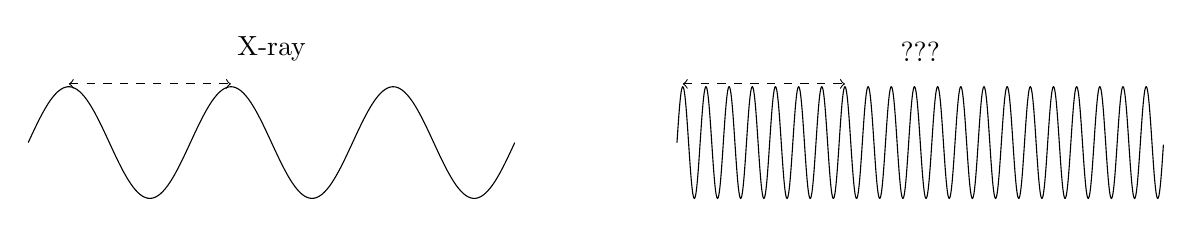
\begin{tikzpicture}
\begin{axis}[width=16cm,height=3cm,
    xmin=0,xmax=14,
    ymin=-1,ymax=1,
    clip=false,
    ticks=none,
    axis line style={draw=none}
    ]
    \draw[dashed,<->] (0.5,1.05) -- ++(axis direction cs: 2,0);
    \draw plot[domain=0:6*pi, samples=200] (\x/pi,{sin(\x r)});
    \node[above=2mm] at (3,1) {X-ray};
    \begin{scope}[shift={(axis direction cs: 8,0)}]
        \draw plot[domain=0:6*pi, samples=1200] (\x/pi,{sin(7/1*\x r)});
        \draw[dashed,<->] (0.5*1/7,1.05) -- ++(axis direction cs: 2,0);
        \node[above=2mm] at (3,1) {???};    
    \end{scope}
\end{axis}
\end{tikzpicture}
\end{center}

\question
The first wave represents a microwave. If the second wave is an a different region of the spectrum, what type of electromagnetic wave is it?


\begin{center}
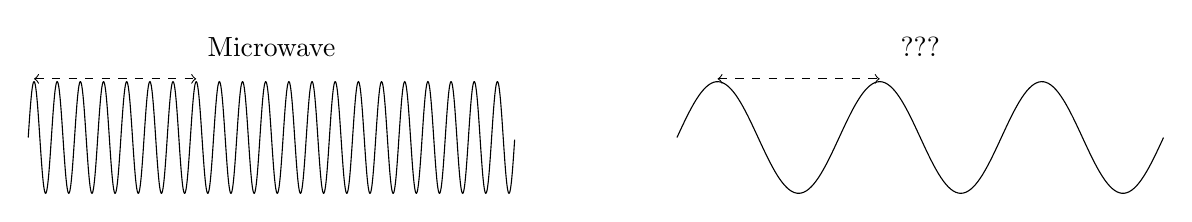
\begin{tikzpicture}
\begin{axis}[width=16cm,height=3cm,
    xmin=0,xmax=14,
    ymin=-1,ymax=1,
    clip=false,
    ticks=none,
    axis line style={draw=none}
    ]
    \draw plot[domain=0:6*pi, samples=1200] (\x/pi,{sin(7/1*\x r)});
    \draw[dashed,<->] (0.5*1/7,1.05) -- ++(axis direction cs: 2,0);
    \node[above=2mm] at (3,1) {Microwave};
    \begin{scope}[shift={(axis direction cs: 8,0)}]
        \draw plot[domain=0:6*pi, samples=200] (\x/pi,{sin(\x r)});
        \draw[dashed,<->] (0.5,1.05) -- ++(axis direction cs: 2,0);
        \node[above=2mm] at (3,1) {???};    
    \end{scope}
\end{axis}
\end{tikzpicture}
\end{center}

\question \label{wqaTm6}
When water molecules are bathed in electromagnetic radiation at just the right frequency, they get begin to vibrate and give off heat to their environment. What frequency must these waves have for this phenomenon to occur? Write the number in scientific and decimal notation.


\question
To what region of the electromagnetic spectrum do the waves from Exercise \ref{wqaTm6} belong? 


\question
What happens to the energy of electromagnetic radiation as frequency decreases?


\question
How do humans detect infrared radiation?


\question
Explain some applications of microwaves in astronomy. 


\question
Which type of electromagnetic wave has the longest wavelength of the whole spectrum?


\question
In what medical technology are radio waves used?

\question
Which type of electromagnetic radiation has the shortest wavelengths?


\question
Which form of EM radiation has the most penetrating ability?


\question
Why are high-frequency gamma rays more dangerous to humans than visible light?
\end{questions}


\subsection{Visible Light}

\begin{questions}


\question
Explain Roy G.~Biv.


\question
Identify the name of the cells in your eyes that allow you to perceive color.


\question
What are the seven colors of the rainbow in order of increasing \textit{wavelength}?


\question
Between red and violet, which color represents the high-frequency limit of the visible spectrum?


\question
Which color represents the long-wavelength limit of the visible spectrum?


\question
Which region of the electromagnetic spectrum, apart from visible light, can bees see?


\question
Which animal can see infrared light?


\question \label{lwLSKO}
Sort the colors yellow, blue, and red from shortest wavelength to longest.


\question
The first wave below represents the electromagnetic wave associated with the color cyan, also known as aqua blue. The second wave represents a different color of the visible light spectrum. Which colors can you rule \textit{out} to be represented by the second wave? Assume that the dashed double arrows are the same length and that cyan lies between green and blue.


\begin{center}
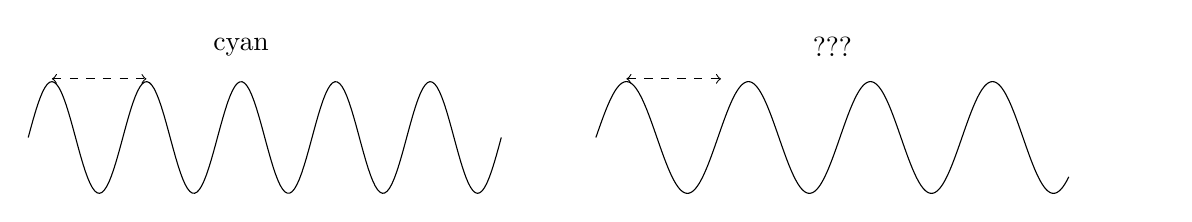
\begin{tikzpicture}
\begin{axis}[width=16cm,height=3cm,
    xmin=0,xmax=24,
    ymin=-1,ymax=1,
    clip=false,
    ticks=none,
    axis line style={draw=none}
    ]
    \draw[dashed,<->] (0.5,1.05) -- ++(axis direction cs: 2,0);
    \draw plot[domain=0:10*pi, samples=200] (\x/pi,{sin(\x r)});
    \node[above=2mm] at (4.5,1) {cyan};
    \begin{scope}[shift={(axis direction cs: 12,0)}]
        \draw[dashed,<->] (0.5*632/490,1.05) -- ++(axis direction cs: 2,0);
        \draw plot[domain=0:10*pi, samples=500] (\x/pi,{sin(490/632*\x r)});
        \node[above=2mm] at (5,1) {???};    
    \end{scope}
\end{axis}
\end{tikzpicture}

\vspace{1em}

% \begin{tikzpicture}
%     \begin{axis}[width=14cm, height=7cm,
%         ymin=0,ymax=1,
%         height=3cm,
%         xmin=360,xmax=740,
%         yticklabels={},
%         ytick=\empty,
%         axis lines=left,
%         separate axis lines,
%         y axis line style=white,
%         x dir=reverse,
%         clip=false,
%         ticks=none,
%         axis line style={draw=none}
%         ]
%         \addplot[draw=none, name path=uv, forget plot] coordinates{(360,0)(360,0.5)};
%         \addplot[draw=none, name path=visible, forget plot] coordinates{(740,0)(740,0.5)};
%         \addplot[shading=visiblelight, area legend] fill between[of=uv and visible];
%         \draw[<-,thick] (490,0.5) -- ++(axis direction cs: 0,0.4) node[above] {cyan};
%     \end{axis}
% \end{tikzpicture}
\end{center}

\question
Convert \SI{5798}{nm} to meters, writing in scientific notation.


\question
Sort the colors in Exercises \ref{lwLSKO} from lowest frequency to highest.


\question
What is the wavelength of a red light wave that has a frequency of \SI{4.746e14}{\Hz} if the wave travels through empty space at a speed of \SI{3.0e8}{m/s}? Express your answer in nanometers (nm).


\question
The Bacillus is a species of rod-shaped bacteria that are very common in nature. As shown below, a typical length is about 2 to 6 microns. Consider a green light wave, which has a wavelength of about 500 nanometers. About how many wave cycles of green light could fit along the length of the Bacillus below?



\begin{center}
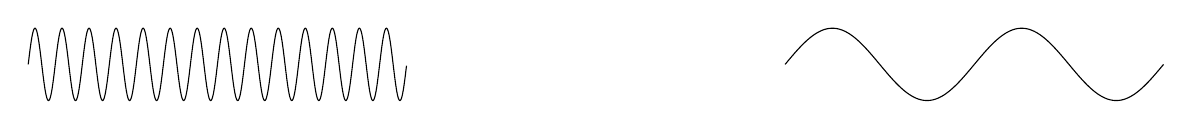
\begin{tikzpicture}
\begin{axis}[width=16cm,height=2.5cm,
    xmin=0,xmax=12,
    ymin=-1,ymax=1,
    clip=false,
    ticks=none,
    axis line style={draw=none}
    ]
    \draw plot[domain=0:4*pi, samples=1200] (\x/pi,{sin(7/1*\x r)});
    \begin{scope}[shift={(axis direction cs: 8,0)}]
        \draw plot[domain=0:4*pi, samples=200] (\x/pi,{sin(\x r)});   
    \end{scope}
\end{axis}
\end{tikzpicture}

\vspace{-1.5cm}

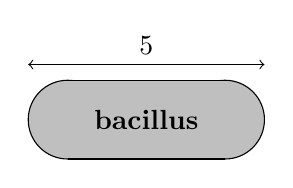
\begin{tikzpicture}
    \draw[fill=lightgray] (0,0) circle (0.5);
    \begin{scope}[shift={(2,0)}]
        \draw[fill=lightgray] (0,0) circle (0.5); 
    \end{scope}
    \fill[lightgray] (0,-0.5) rectangle ++(2,1) node[black,pos=0.5] {\textbf{bacillus}};
    \draw (0,0.5) -- ++(2,0)
          (0,-0.5) -- ++(2,0);
    \draw[<->] (-0.5,0.7) -- ++(3,0) node[above,pos=0.5] {\SI{5}{\micro\meter}};
\end{tikzpicture}
\end{center}


\question
True or false? Light requires a medium to propagate.


\question
What is the value of $c$, the speed of light in a vacuum?


\question
Saturn is \SI{1.43e12}{m} from the Sun. How many minutes does it take the Sun’s light to reach Saturn? To get full credit, show all your work.
\end{questions}

\subsection{Optics}

\end{document}

